\section{Ejercicios}
	
	\begin{enumerate}
		
\item Calcular la impedancia equivalente $\overline{Z_{eq}}$ del circuito de la Figura \ref{fig.ej_CA1}, expresándolo en forma binaria y polar.
 \begin{figure}[H]
        \centering
        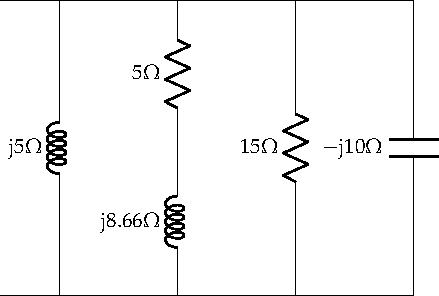
\includegraphics[width=0.35\linewidth]{../figs/ej1_BT2.pdf}
        \caption{Ejercicio 1}
        \label{fig.ej_CA1}
    \end{figure}
    \emph{Sol.: $\overline{Z_{eq}}=4.54\phase{57.9855^\circ}\Omega=2.41+\mathrm{j}3.85\Omega$}
    \item Determinar $\overline{Z}$ en el circuito de la Figura \ref{fig.ej_CA2}.
     \begin{figure}[H]
        \centering
        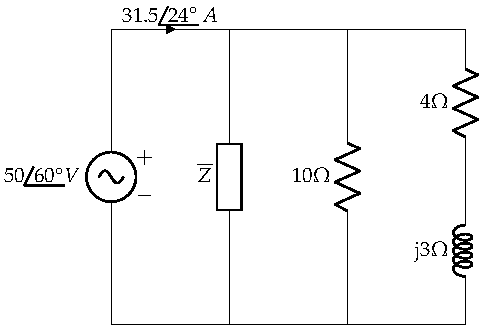
\includegraphics[width=0.5\linewidth]{../figs/ej2_BT2.pdf}
        \caption{Ejercicio 2}
        \label{fig.ej_CA2}
    \end{figure}
    \emph{Sol.: $\overline{Z}=2.83\phase{45.0715^\circ}\Omega$}
    \item Un circuito serie con dos elementos consume una potencia activa de $940$ W y tiene un factor de potencia $0.707$ en $adelanto$. Determinar los elementos del circuito si la tensión tiene un valor máximo $99$ V. \\
    \emph{Sol.: $R=2.60\Omega;\;C=1.22\,mF$}
    \item Un circuito en serie con una resistencia $10\Omega$ y una inductancia $\mathrm{j}5\Omega$ tiene una tensión eficaz aplicada de $120$ V. Determinar las potencias consumidas y el factor de potencia, indicando si éste va en retraso o adelanto. \\
    \emph{Sol.: $P=1151.33 \,W;\; Q=575.66 \,VAr;\; \overline{S}=1287.22\phase{26.5649^\circ} VA;\; \cos(\phi)=0.894$, en retraso}
    \item Para determinar las constantes $R$ y $L$ de una bobina, se conecta en serie con una resistencia de {25}{$\Omega$} y al conjunto se le aplica una fuente de tensión de {120}{V} a {60}{Hz}, se miden las tensiones en bornes de la resistencia y de la bobina, dando los valores $U_R = {70.8}{V}$ y $U_B = {86}{V}$. ¿Cuáles son las constantes de la bobina?\\
    \emph{Sol.: $R= 5{\Omega};\; L = {79.5}mH$}
    \item En un circuito serie $RL$ con $R=5\Omega$ y $L=0.06H$, la tensión en bornes de la bobina es $u_L(t)=15\sin(200\,t)$ V. Determinar:
    \begin{itemize}
        \item La tensión total
        \item Intensidad de corriente
        \item Ángulo de desfase de la intensidad respecto de la tensión
        \item Impedancia del circuito
    \end{itemize}
    \emph{Sol.: $\overline{Z_{eq}}=5+\mathrm{j}\,12\Omega;\;\overline{I}=0.88\phase{-90^\circ}A;\;\overline{U}=11.48\phase{-22.5304^\circ} V;\; \phi=67.4696^\circ$}
    \item Un circuito serie RLC con $R = {5}{\Omega}$ , $L = {0.02}{H}$ y $C={80}{\mu F}$, tiene aplicada una tensión senoidal de frecuencia variable. Determinar los valores de la pulsación $\omega$ para los cuales la corriente:
\begin{itemize}
\item Adelanta {45}{$^\circ$} a la tensión
\item Está en fase con ella
\item Retrasa {45}{$^\circ$}
\end{itemize}
\emph{Sol.: $\omega=675.39\,rad/s;\; \omega=790.57\,rad/s;\, \omega=925.39\,rad/s$}
\item Determinar el triángulo de potencias de un circuito al que se le aplica una tensión $u(t)=340 \cdot \sin(\omega t - 60^\circ)$ V y circula una intensidad de corriente $i(t)= 13.3 \cdot \sin(\omega t-48.7^\circ)$.\\
\emph{Sol.: $P=2217.17\,W;\;Q=443.03\,VAr;\;S=2261\phase{-11.3^\circ}\,VA$}
\item En el esquema de la Figura~\ref{fig.ej8_BT2} los elementos tienen los siguientes valores:
\begin{align*}
    R_1 &= R_2 = R_3 = {10}{\Omega}\\
    X_1 &= X_2 = {1}{\Omega}\\
    R_L &= X_L = {1}{\Omega}
\end{align*}
Sabiendo que $U_{CD} = {200}{V}$ se debe calcular:
\begin{itemize}
\item Intensidades de corriente $I$, $I_1$, $I_2$ e $I_3$ {en forma fasorial}, tomando $U_{CD}$ como referencia de fase
\item Lectura de los vatímetros $W_1$ y $W_2$
\end{itemize}
\begin{figure}[H]
    \centering
    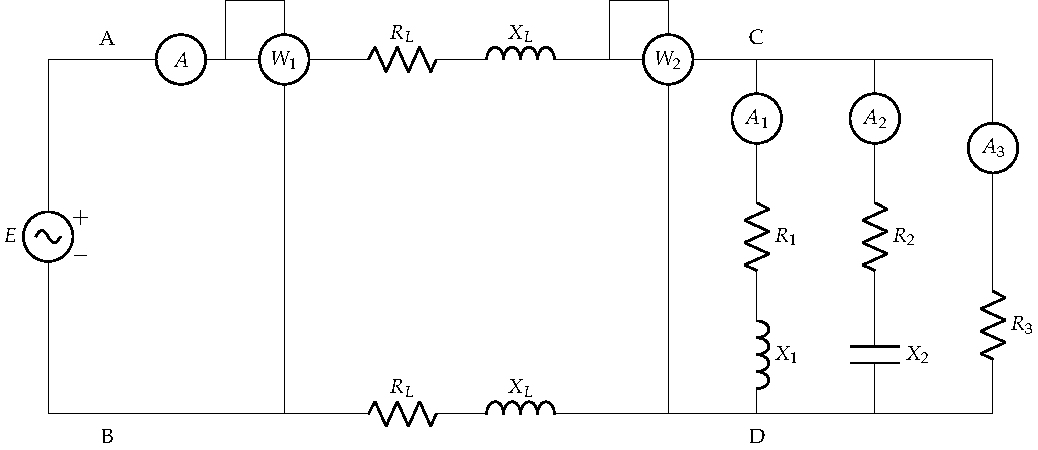
\includegraphics[width=\linewidth]{../figs/ej8_BT2.pdf}
    \caption{Ejercicio 9}
    \label{fig.ej8_BT2}
\end{figure}
\emph{Sol.: $\overline{I_1}=19.90\phase{-5.7106^\circ}\,A;\; \overline{I_2}=19.90\phase{5.7106^\circ}\,A;\; \overline{I_3}=20\phase{0^\circ}\,A;\;\overline{I}=59.60\phase{0^\circ}\,A;\;W_1=19024.32\,W;\; W_2=11920\,W$}
\item En el circuito de la Figura~\ref{fig.ej9_BT2}, los amperímetros $A_1$ y $A_2$ marcan ${4.5}{A}$ y ${6}{A}$, respectivamente; el voltímetro, ${150}{V}$ y el vatímetro ${900}{W}$. Sabiendo que la frecuencia del generador es de ${250}{Hz}$ y el f.d.p. de la impedancia $Z$ es de 0.8 en retraso, se pide calcular:
\begin{itemize}
\item Valores de R, C y Z en forma compleja
\item La tensión del generador
\end{itemize}
\begin{figure}[H]
    \centering
    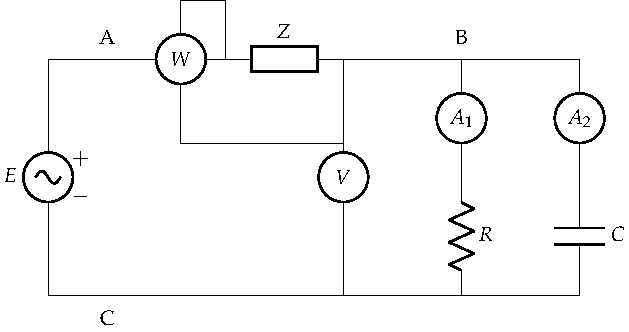
\includegraphics{../figs/ej9_BT2.pdf}
    \caption{Ejercicio 10}
    \label{fig.ej9_BT2}
\end{figure}
\emph{Sol.: $\overline{R}=33.33\phase{0^\circ}\Omega; \,\overline{X_c}-\mathrm{j}\,25\Omega;\,\overline{Z}=16+\mathrm{j}\,12\Omega;\,\overline{U_{AC}}=212.13\phase{45^\circ} V$}
\item En el circuito de la Figura~\ref{fig.ej11_BT2}, determinar las lecturas de los aparatos de medida y el balance de potencias activas y reactivas, así como el triángulo global de potencias.\\
Datos: $e(t)=100\sqrt{2}(\omega\,t)$; $R_1=2\Omega$; $R_2=4\Omega$; $\omega\,L=4\Omega$.
\begin{figure}[H]
    \centering
    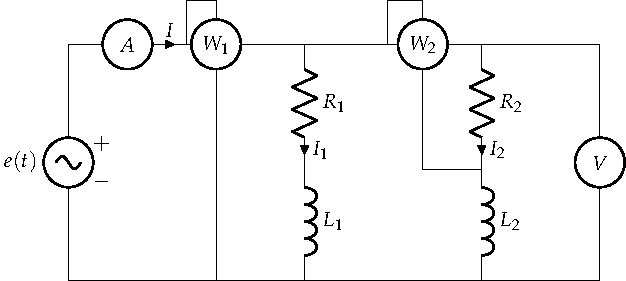
\includegraphics{../figs/ej11_BT2.pdf}
    \caption{Ejercicio 11}
    \label{fig.ej11_BT2}
\end{figure}
\emph{Sol.: $V=100\,V;\;A = 45.20 A;\;W_1=2788.31W;\;W_2=1250.33\,W;\,P_{R1}=1539.02 W;\;P_{R2}=1250.33 W;\,Q_{L1}=2308.52 VAr;\;Q_{L2}=1250.33 VAr;\,P_T=2789.35 W;\,Q_T=3558.82 VAr;\;\overline{S_T}=2789.35+\mathrm{j}3558.82 VA$}
\item Un motor monofásico de $S = {10}{kVA}$ y $fdp = 0.8$ está alimentado por una fuente de ${230}{V}$ a $f = {50}{Hz}$.
Calcular:
\begin{itemize}
    \item El valor eficaz de la corriente absorbida por el motor
    \item La potencia aparente del generador
    \item La capacidad del condensador necesario para compensar el factor de potencia a la unidad
    \item El valor eficaz de la corriente absorbida por el conjunto condensador-motor
    \item La potencia aparente del generador necesario una vez conectado el condensador del tercer apartado
    \item Compara de forma razonada los resultados de los apartados 4 y 5 con los valores calculados en los apartados 1 y 2
\end{itemize}
\emph{Sol.: $I= {43.5}{A};\; S_g = {10}{kVA};\;C={361}{\mu F};\, I'=34.78A;\, S_g' = {8000}{kVA}$}

\item Un generador de corriente alterna monofásica ($f=50$ Hz) alimenta a dos cargas a través de una línea de cobre. Esta línea, de resistividad $\rho=21$ m$\Omega$ mm$^2$/m, tiene una longitud de 100 m y una sección de 16 mm$^2$. Las dos cargas, cuya tensión de alimentación es de 230 V, son dos motores, uno con potencia de 7 kW y f.d.p. de $0.65$, y otro con una potencia de 5 kW y f.d.p. de $0.85$. Con esta información, se pide calcular:
\begin{itemize}
    \item Triángulo de potencias de cada carga y del conjunto de ambas
    \item Valor eficaz de las corrientes en cada carga y de la corriente total
    \item Triángulo de potencias del generador
    \item Valor eficaz de la tensión en bornes del generador
    \item Capacidad del condensador a instalar en bornes de las cargas para mejorar el factor de potencia a $0.95$
    \item Valor eficaz de la corriente entregada por el generador una vez instalado el condensador
    \item Triángulo de potencias del generador una vez instalado el condensador
\end{itemize}
\emph{Sol.: $P_1=7000W;\; Q_1=8183.91VAr;\;S_1=10769.23VA;\;P_2=5000W;\;Q_2=5882.35VAr;\;S_2=3098.72VA;\;P_T=12000W;\;Q_T=11282.63VAr;\;S_T=16471.12VA;\, I_1=46.82\,A;\;I_2=25.58\,A;\;I_T=71.62\,A;\,P_g=13333.65 W;\;Q_g=11282.63 VAr;\,S_g=17466.65 VA;\;U_g=243.88 V;\; C=441.66 \mu F;\,I'=54.92 A;\;P_g'=12784.21 W;\;Q_g'=3944.21 VAr;\;S_g'=13378.82 VA$}
\item Determinar la capacidad del condensador de la Figura~\ref{fig.ejemplo9_BT2} para que la corriente de la fuente esté en fase con la tensión de alimentación, sabiendo que $f=50$ Hz.
	    \begin{figure}[H]
	        \centering
	        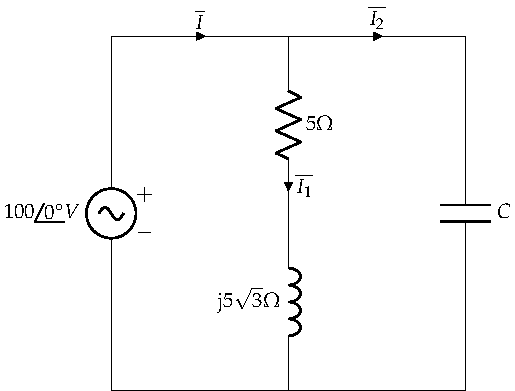
\includegraphics{../figs/ejemplo9_BT2.pdf}
	        \caption{Ejercicio 14}
	        \label{fig.ejemplo9_BT2}
	    \end{figure}
\emph{Sol.: $C=275.59\,\mu F$}
\item Calcular la corriente $i(t)$ del circuito de la Figura~\ref{fig.ejercicio13_BT2}.
\begin{figure}[H]
    \centering
    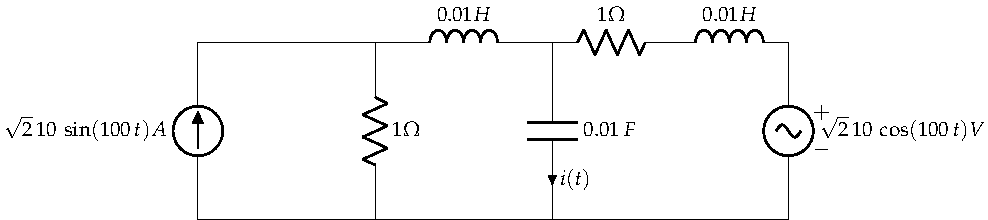
\includegraphics[width=\linewidth]{../figs/ejercicio13_BT2.pdf}
    \caption{Ejercicio 15}
    \label{fig.ejercicio13_BT2}
\end{figure}
\emph{Sol.: $i(t)=\sqrt{2}\,10\,\cos(100\,t) A$}

\item Un generador de corriente alterna monofásica ($f = {50}{Hz}$) alimenta a dos cargas a través de una línea de cobre. Esta línea, de resistividad $\rho = {0.017}{\Omega mm^2/m}$, tiene una longitud de {40}{m} y una sección de {6}{mm$^2$}. Las dos cargas, cuya tensión de alimentación es de {200}{V}, son:
\begin{enumerate}
\item Un motor de {7}{kW} con f.d.p. {0,7}.
\item Un grupo de lámparas fluorescentes con potencia total {200}{W} y f.d.p. {0,5}.
\end{enumerate}
Se pide: 
\begin{itemize}
    \item Esquema del circuito señalando adecuadamente los elementos, corrientes y tensiones
    \item Potencias activa, reactiva y aparente de cada carga
    \item Valor eficaz de las corrientes en cada carga, y de la corriente total
    \item Potencia activa y reactiva entregada por el generador
    \item Valor eficaz de la tensión en bornes del generador
    \item Capacidad necesaria a instalar en bornes de las cargas para mejorar el factor de potencia de las mismas a la unidad
    \item Valor eficaz de la tensión en bornes del generador, y potencia aparente entregada por el mismo una vez instalada la capacidad determinada en el apartado anterior
\end{itemize}
\emph{Sol.: $P_M = {7000}{W};\; Q_M = {7141.43}{VAr};\; S_M ={10000}{VA};\; P_F = {200}{W};\;  Q_F = {346.41}{VAr};\; S_F ={400}{VA};\;I_M = {50}{A};\; I_F = {2}{A};\; I_T = {51.94}{A};\;P_g = {7811.50}{W};\; Q_g = {7487.8}{VAr};\; U_g = {208.33}{V}; C={595.86}{\mu F};\; U_g' = {207.92}{V};\; S_g' = {7485.12}{VA}$ }
\item El circuito de la Figura~\ref{fig.ej17_BT2} tiene carácter inductivo.  La impedancia de la línea es $Z={10\sqrt{2}}{\Omega}$ con
f.d.p. $\sqrt{2}/2$ en retraso. Tomando como referencia de fases la intensidad total $\overline{I}$, se pide calcular:
\begin{itemize}
\item Potencia activa y reactiva consumida por $Z$
\item Expresiones complejas de las intensidades medidas por los amperímetros $A$, $A_1$, $A_2$ y $A_3$ 
\item  Expresiones complejas de las tensiones $\overline{U_{AB}}$, $\overline{U_{AC}}$ y $\overline{U_{CB}}$
\item  Valores de $R_1$, $X_1$, $R_2$, $R_3$ y $X_3$
\end{itemize}
Datos: $A = {5\sqrt{5}}{A};\; A_1 = {5\sqrt{2}}{A};\;A_2 = {5}{A};\;A_3 = {\sqrt{10}}{A};\;U_{AB} = {247}{V};\;W_1 = {2350}{W};\;R_1 = R_3$
\begin{figure}[H]
    \centering
    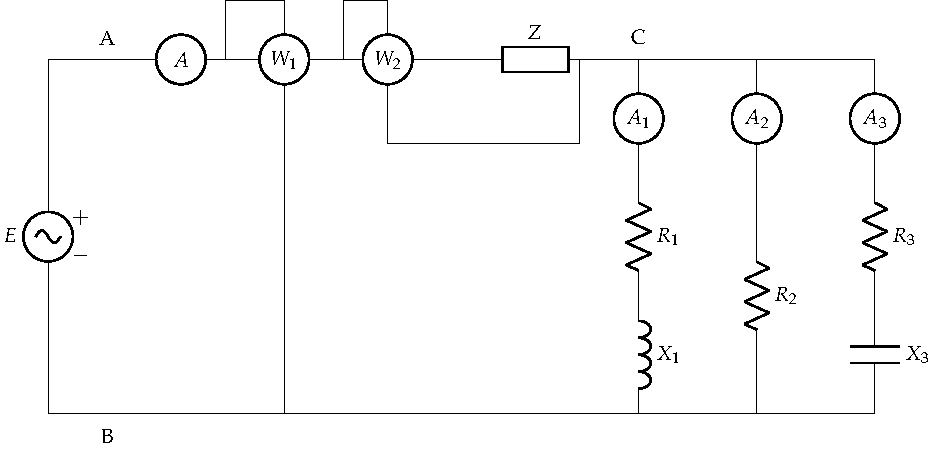
\includegraphics[width=0.8\linewidth]{../figs/ej17_BT2.pdf}
    \caption{Ejercicio 17}
    \label{fig.ej17_BT2}
\end{figure}
\emph{Sol.: $P_z=1250\,W;\;Q_z=1250\,VAr;\;\overline{I}=11.18\phase{0^\circ}A;\; \overline{I_1}=7.07\phase{-34.6711^\circ}A;\; \overline{I_2}=5\phase{10.3289^\circ}A;\;\overline{I_3}=3.16\phase{81.8940^\circ}A;\; \overline{U_{AB}}=247\phase{31.6823^\circ}V;\; \overline{U_{AC}}=158.11\phase{45^\circ}\,V;\; \overline{U_{CB}}=100\phase{10.3289^\circ} V;\;R_1=R_3=10\Omega;\;R_2=20\Omega; X_1=10\Omega;\;X_3=-30\Omega$}

\item {Del circuito de la Figura~\ref{fig.ej18_BT2}, obtener:
    \begin{itemize}
        \item Expresiones analíticas de las intensidades $i_1(t)$ e $i_2(t)$
        \item Potencia disipada por todas las resistencias
    \end{itemize}}
Datos: $e_g(t)=50\sqrt{2}\sin(1000\,t)$ V; $i_g(t)=10$ A; $R_1=R_2=2\Omega$; $R_3=7\Omega$; $L_1=L_2=1$ mH; $L_3=2$ mH
\begin{figure}[H]
    \centering
    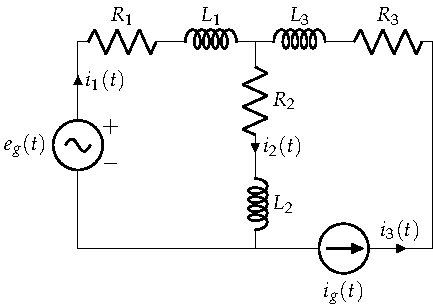
\includegraphics{../figs/ej18_BT2.pdf}
    \caption{Ejercicio 18}
    \label{fig.ej18_BT2}
\end{figure}
\emph{Sol.: $i_1(t)= -5+5\sqrt{10}\sin(1000t-0.46) A;\; i_2(t)= 5+5\sqrt{10}\sin(1000t-0.46) A;\; i_3(t)= 10 A;\; P_T=1300\,W$}

\item Del esquema de la Figura~\ref{fig.ej19_BT2} hallar:
    \begin{itemize}
        \item Equivalente de Thévenin del circuito situado a la izquierda de los terminales de $A-B$ 
        \item Potencia disipada por la impedancia conectada a la derecha de los terminales $A-B$
        \item Impedancia a conectar al equivalente de Thévenin para que éste entregue la máxima potencia, así como dicha potencia
    \end{itemize}
    Datos: $u(t)=80\sqrt{2}\sin(t+\frac{\pi}{2})$ V;          $R_1=R_2=2\Omega$;          $R_3=3\Omega$;          $L_1=3$ H;         $L_2=2$ H;   $C_1=1$ F;            $C_2=0.2$ F
    \begin{figure}[H]
        \centering
        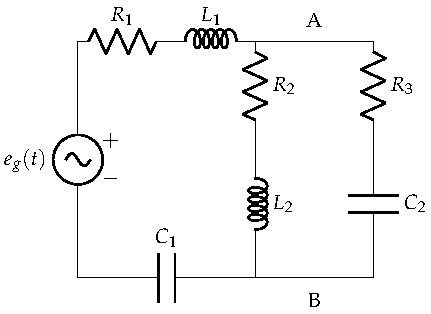
\includegraphics{../figs/ej19_BT2.pdf}
        \caption{Ejercicio 19}
        \label{fig.ej19_BT2}
    \end{figure}
    \emph{Sol.: $\overline{E_{th}}=40\phase{90^\circ}\,V;\;\overline{Z_{th}}=1+\mathrm{j}\,\Omega;\,P_{R3}=150\,W;\, \overline{Z_L} = 1-\mathrm{j} \;\Omega; P_{max} = 400\,W$}
    
    \item En el circuito de la Figura~\ref{fig.superposicion2_ej} determina:
\begin{itemize}
\item $u_R(t)$  y $u_L(t)$
\item Balance de potencias
\end{itemize}
Datos: $e_a(t) = {3\sqrt{2} \sin(10^3 t)} V;\,e_b(t) = {30\sqrt{2} \sin(10^4 t)} V;\,R = {30}{\Omega};\,L = {3}{mH}$
\begin{figure}[H]
    \centering
    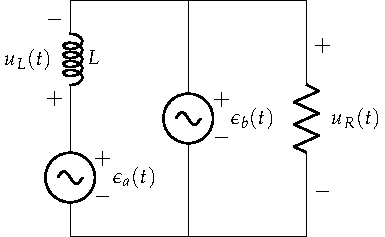
\includegraphics{../figs/superposicion2_ej.pdf}
    \caption{Ejercicio 20}
    \label{fig.superposicion2_ej}
\end{figure}
\emph{Sol.: $u_R(t) =  30\sqrt{2}\sin(10^4 t) V;\; u_L(t) = 3\sqrt{2}\sin(10^3 t) - 30\sqrt{2}\sin(10^4 t) V;\; P_R = {30}{W};\; P_\epsilon = {-30}{W}$}

\item El circuito de la Figura~\ref{fig.ej21_BT2} se encuentra en régimen permanente. Determinar analíticamente la expresión de $i(t)$, así como las potencias entregadas por los generadores y disipadas por las resistencias $R_1$ y $R_2$.

Datos: $e_1(t) = {50 \sin(1000 t)} V;\; e_2(t) = {30}{V};\; R_1 = {6}{\Omega};\; R_2 = {6}{\Omega};\; L = {8}{mH};\; C = {10}{\mu F}$

\begin{figure}[H]
    \centering
    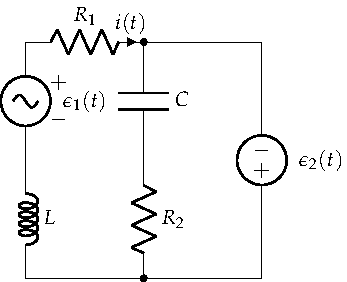
\includegraphics{../figs/superposicion1_ej.pdf}
    \caption{Ejercicio 21}
    \label{fig.ej21_BT2}
\end{figure}

\emph{Sol.: $i(t) = 5 + 5\sin(1000t - 0.9273){A};\; P_{R1} = {225}{W}; P_{R2} = {0}{W}; P_{\epsilon} = -{225}{W}$}

\item Obtener el generador equivalente de Thévenin del circuito de la Figura~\ref{fig.ej22_BT2} respecto de A y B.\\
Datos: $\overline{\epsilon_g} = {12 - \mathrm{j}16}{V};\, \overline{Z}_1 = {1 - \mathrm{j}}{\Omega};\; \overline{Z}_2 = {1 + \mathrm{j}}{\Omega};\; \overline{Z}_3 = {5 + \mathrm{j}3}{\Omega};\; \alpha = 2$

\begin{figure}[H]
    \centering
    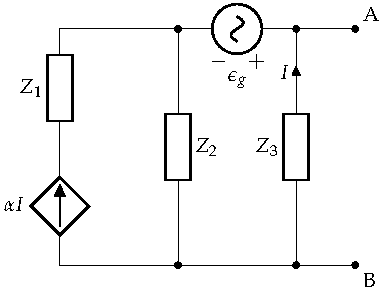
\includegraphics{../figs/Thevenin4.pdf}
    \caption{Ejercicio 22}
    \label{fig.ej22_BT2}
\end{figure}

\emph{Sol.: $\overline{\epsilon_{th}}=6 - \mathrm{j}10\,V;\;\overline{Z_{th}}=0.64 + \mathrm{j} 0.52{\Omega}$}

\end{enumerate}
%%% Local Variables:
%%% mode: latex
%%% TeX-master: "enunciados_ejercicios_TC"
%%% ispell-local-dictionary: "castellano"
%%% End:
